% IntentDiT architecture (Figure 2), version 3.
% Compile: pdflatex fig02_architecture_v3.tex (in fig/src) or plot_architecture_v3.tex (in code/scripts).
% Output width: exactly 18.47 cm (the MDPI full width), including the surrounding white margin.
% Thumbnails (relative to this file): arch/input.png, arch/saliency.png, arch/placement.png, arch/output.png.
% A labeled fallback appears only if a thumbnail is missing.
% The decoder's x4 group replaces the long repetition arrow; it is not a
% change to the model. All modules, branches, and loss-gating rules are kept.
\documentclass[border=0pt]{standalone}
\usepackage{tikz}
\usepackage[T1]{fontenc}
\usepackage{amsmath,amssymb,graphicx}
\usepackage{mathpazo}
\usepackage[scaled=0.95]{helvet}
\renewcommand{\familydefault}{\sfdefault}
\usetikzlibrary{arrows.meta,calc,backgrounds}

% The pathway palette follows the supplied figure.
\definecolor{inp}{HTML}{4A7FC1}
\definecolor{grn}{HTML}{5A9E4B}
\definecolor{org}{HTML}{D98C2B}
\definecolor{pur}{HTML}{8B68B8}
\definecolor{ind}{HTML}{5F67B8}
\definecolor{red}{HTML}{C9504C}
\definecolor{ink}{HTML}{26313B}
\definecolor{muted}{HTML}{64717D}
\definecolor{rule}{HTML}{DCE2E8}

% Fonts are about 90% of these sizes after the full-width resize below.
\newcommand{\fHead}{\fontsize{10.5}{12.2}\selectfont\bfseries}
\newcommand{\fMain}{\fontsize{8.0}{9.4}\selectfont}
\newcommand{\fBold}{\fMain\bfseries}
\newcommand{\fSmall}{\fontsize{6.9}{8.1}\selectfont}
\newcommand{\fTiny}{\fontsize{6.1}{7.1}\selectfont}

\tikzset{
  >={Stealth[length=1.65mm,width=1.25mm]},
  wire/.style={draw=ink,line width=0.60pt,line cap=round,line join=round},
  arr/.style={wire,->},
  route/.style={wire,draw=#1!90!black},
  flow/.style={route=#1,->},
  crossing/.style={preaction={draw=white,line width=2.7pt,-}},
  panel/.style={draw=#1!75,fill=#1!5,rounded corners=3pt,line width=0.60pt},
  input/.style={panel=#1,minimum width=3.00cm,inner sep=0pt},
  cell/.style={draw=#1!85,fill=white,rounded corners=2pt,line width=0.55pt,
    align=center,text=ink,font=\fMain,inner xsep=2pt,inner ysep=2pt},
  module/.style={cell=pur,minimum width=3.90cm,text width=3.68cm,
    minimum height=0.76cm},
  head/.style={font=\fHead,text=ink,anchor=base},
  note/.style={font=\fSmall,text=muted,align=center,inner sep=1pt},
  junction/.style={circle,fill=#1,draw=none,minimum size=2.7pt,inner sep=0pt}
}

% #1 file; #2 maximum width; #3 maximum height; #4 accent; #5 symbol.
% Bounding both dimensions prevents wide thumbnails from covering labels.
\newcommand{\Asset}[5]{%
  \IfFileExists{#1}{%
    \includegraphics[width=#2cm,height=#3cm,keepaspectratio]{#1}%
  }{%
    \begin{tikzpicture}[x=1cm,y=1cm,baseline=(current bounding box.center)]
      \draw[draw=#4!45,fill=white,rounded corners=1.5pt,
            dash pattern=on 1.5pt off 1.2pt,line width=0.45pt]
        (0,0) rectangle (#2,#3);
      \node[text=#4!80!black,font=\fontsize{12}{14}\selectfont,
            inner sep=0pt] at ({#2/2},{#3/2+0.10}) {#5};
      \node[text=muted,font=\fontsize{5.5}{6.3}\selectfont,
            inner sep=0pt] at ({#2/2},{#3/2-0.20}) {no asset};
    \end{tikzpicture}%
  }%
}

\begin{document}
\resizebox{18.47cm}{!}{%
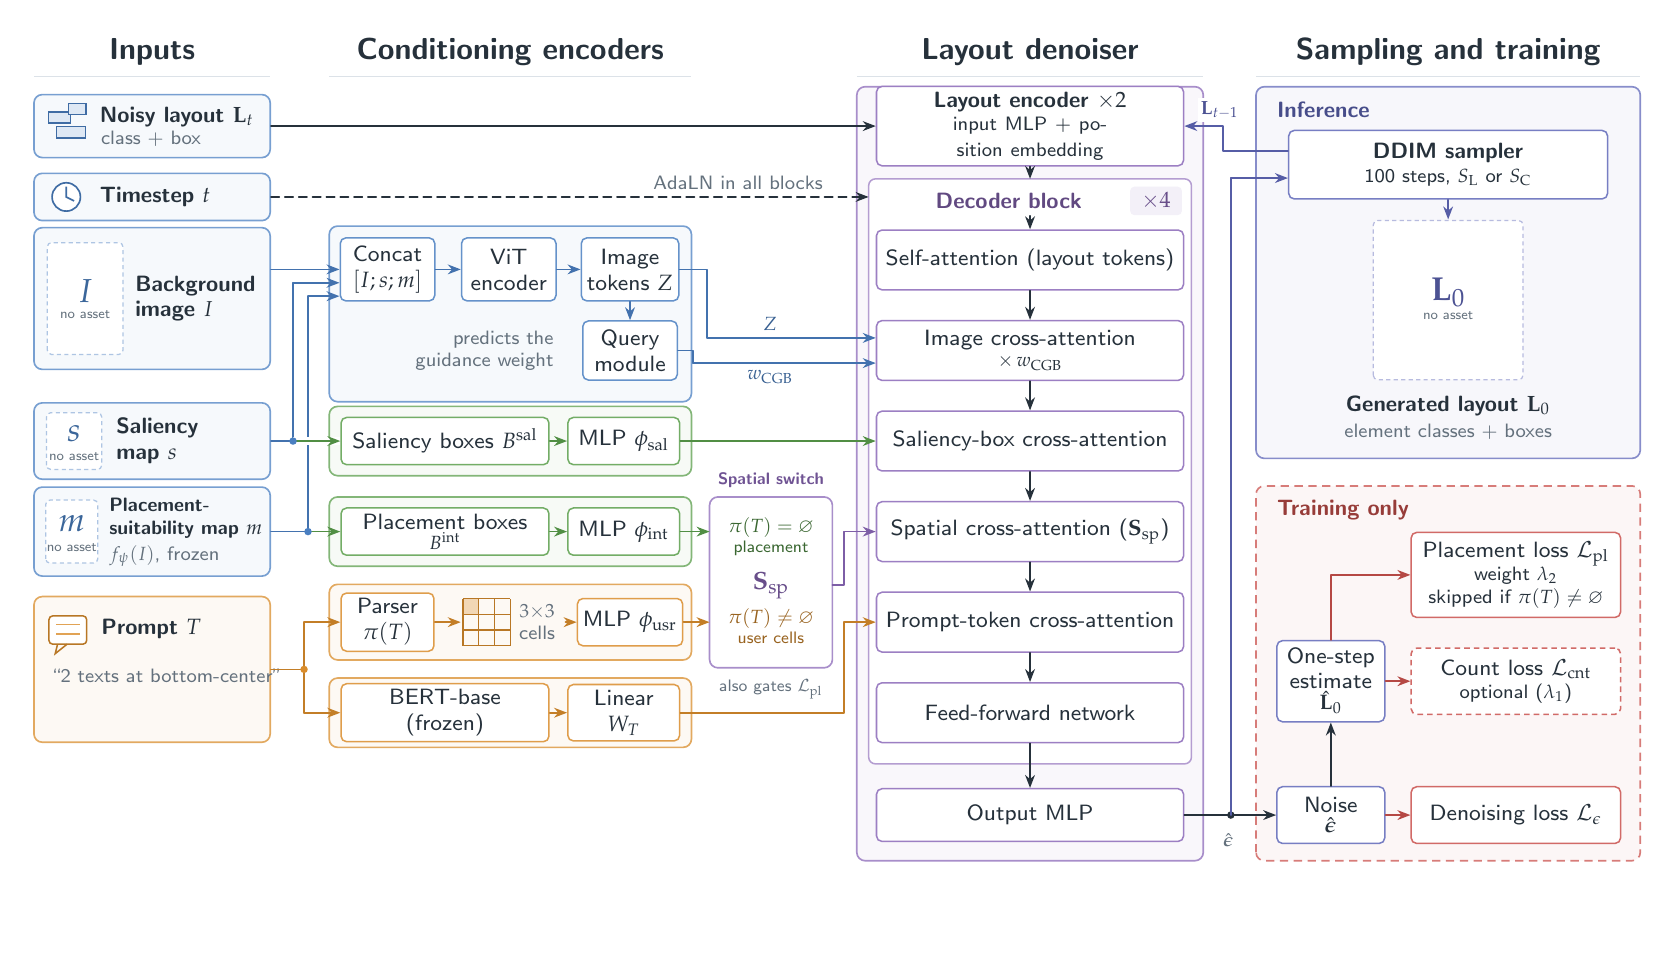
\begin{tikzpicture}[x=1cm,y=1cm]
\path[use as bounding box] (-0.08,-0.06) rectangle (20.48,11.40);

% ------------------------------------------------------------------
% Column grid: inputs | encoders | switch/routing | denoiser | outputs.
% The six decoder stages use a uniform 1.15 cm vertical rhythm.
% ------------------------------------------------------------------
\node[head] at (1.50,10.99) {Inputs};
\node[head] at (6.05,10.99) {Conditioning encoders};
\node[head] at (12.65,10.99) {Layout denoiser};
\node[head] at (17.96,10.99) {Sampling and training};
\draw[draw=rule,line width=0.45pt] (0,10.78) -- (3.00,10.78);
\draw[draw=rule,line width=0.45pt] (3.75,10.78) -- (8.35,10.78);
\draw[draw=rule,line width=0.45pt] (10.45,10.78) -- (14.85,10.78);
\draw[draw=rule,line width=0.45pt] (15.52,10.78) -- (20.40,10.78);

% ------------------------------------------------------------------
% Inputs.
% ------------------------------------------------------------------
\node[input=inp,minimum height=0.80cm] (noisy) at (1.50,10.15) {};
\foreach \x/\y/\w in {0.18/10.19/0.28,0.29/10.00/0.36,0.44/10.30/0.22}
  \draw[draw=inp!85!black,fill=inp!18,line width=0.45pt]
    (\x,\y) rectangle ++(\w,0.14);
\node[font=\fBold,text=ink,anchor=west,inner sep=0pt]
  at (0.83,10.27) {Noisy layout $\mathbf{L}_t$};
\node[note,anchor=west] at (0.81,9.99) {class + box};

\node[input=inp,minimum height=0.60cm] (time) at (1.50,9.25) {};
\draw[draw=inp!85!black,line width=0.6pt,fill=white]
  (0.41,9.25) circle (0.18);
\draw[draw=inp!85!black,line width=0.6pt]
  (0.41,9.38) -- (0.41,9.25) -- (0.51,9.20);
\node[font=\fBold,text=ink,anchor=west,inner sep=0pt]
  at (0.83,9.25) {Timestep $t$};

\node[input=inp,minimum height=1.80cm] (image) at (1.50,7.96) {};
\node[inner sep=0pt] at (0.65,7.96)
  {\Asset{arch/input.png}{0.96}{1.42}{inp}{$I$}};
\node[font=\fontsize{7.8}{9.3}\selectfont\bfseries,text=ink,
      anchor=west,align=left,inner sep=0pt]
  at (1.28,7.96) {Background\\image $I$};

\node[input=inp,minimum height=0.97cm] (saliency) at (1.50,6.15) {};
\node[inner sep=0pt] at (0.51,6.15)
  {\Asset{arch/saliency.png}{0.70}{0.72}{inp}{$s$}};
\node[font=\fBold,text=ink,anchor=west,align=left,inner sep=0pt]
  at (1.04,6.15) {Saliency\\map $s$};

\node[input=inp,minimum height=1.13cm] (placement) at (1.50,5.00) {};
\node[inner sep=0pt] at (0.48,5.00)
  {\Asset{arch/placement.png}{0.66}{0.80}{inp}{$m$}};
\node[font=\fontsize{7.3}{8.6}\selectfont\bfseries,text=ink,
      anchor=west,align=left,inner sep=0pt]
  at (0.95,5.17) {Placement-\\suitability map $m$};
\node[note,anchor=west] at (0.92,4.69) {$f_\psi(I)$, frozen};

\node[input=org,minimum height=1.85cm] (prompt) at (1.50,3.25) {};
\draw[draw=org!85!black,fill=white,line width=0.55pt,rounded corners=1.4pt]
  (0.19,3.57) rectangle (0.67,3.93);
\draw[draw=org!85!black,line width=0.55pt]
  (0.30,3.57) -- (0.27,3.45) -- (0.42,3.57);
\foreach \y in {3.82,3.70}
  \draw[draw=org!80,line width=0.45pt] (0.28,\y) -- (0.58,\y);
\node[font=\fBold,text=ink,anchor=west,inner sep=0pt]
  at (0.85,3.76) {Prompt $T$};
\node[note,anchor=north west,align=left,inner sep=0pt]
  at (0.20,3.26) {``2 texts at bottom-center''};

% ------------------------------------------------------------------
% Conditioning encoders. Each card has a consistent internal margin.
% ------------------------------------------------------------------
\draw[panel=inp] (3.75,6.65) rectangle (8.35,8.88);
\node[cell=inp,minimum width=1.20cm,minimum height=0.80cm]
  (cat) at (4.49,8.33) {Concat\\$[I;s;m]$};
\node[cell=inp,minimum width=1.20cm,minimum height=0.80cm]
  (vit) at (6.03,8.33) {ViT\\encoder};
\node[cell=inp,minimum width=1.20cm,minimum height=0.80cm]
  (Z) at (7.57,8.33) {Image\\tokens $Z$};
\node[cell=inp,minimum width=1.20cm,minimum height=0.75cm]
  (qm) at (7.57,7.30) {Query\\module};
\node[note,anchor=east,align=right] at (6.64,7.30)
  {predicts the\\guidance weight};
\draw[flow=inp] (cat.east) -- (vit.west);
\draw[flow=inp] (vit.east) -- (Z.west);
\draw[flow=inp] (Z.south) -- (qm.north);

\draw[panel=grn] (3.75,5.71) rectangle (8.35,6.59);
\node[cell=grn,minimum width=2.64cm,text width=2.47cm,minimum height=0.60cm]
  (sb) at (5.22,6.15) {Saliency boxes $B^{\mathrm{sal}}$};
\node[cell=grn,minimum width=1.42cm,text width=1.26cm,minimum height=0.60cm]
  (ms) at (7.49,6.15) {MLP $\phi_{\mathrm{sal}}$};
\draw[flow=grn] (sb.east) -- (ms.west);

\draw[panel=grn] (3.75,4.56) rectangle (8.35,5.44);
\node[cell=grn,minimum width=2.64cm,text width=2.47cm,minimum height=0.60cm]
  (pb) at (5.22,5.00) {Placement boxes\\[-2pt]{\fSmall $B^{\mathrm{int}}$}};
\node[cell=grn,minimum width=1.42cm,text width=1.26cm,minimum height=0.60cm]
  (mi) at (7.49,5.00) {MLP $\phi_{\mathrm{int}}$};
\draw[flow=grn] (pb.east) -- (mi.west);

\draw[panel=org] (3.75,3.37) rectangle (8.35,4.33);
\node[cell=org,minimum width=1.18cm,minimum height=0.66cm]
  (pp) at (4.49,3.85) {Parser\\$\pi(T)$};
\begin{scope}[shift={(5.45,3.55)}]
  \fill[org!35] (0,0.40) rectangle (0.20,0.60);
  \draw[draw=org!85!black,line width=0.45pt]
    (0,0) grid[step=0.20] (0.60,0.60);
\end{scope}
\node[note] at (6.39,3.85) {$3{\times}3$\\cells};
\node[cell=org,minimum width=1.26cm,minimum height=0.60cm]
  (mu) at (7.57,3.85) {MLP $\phi_{\mathrm{usr}}$};
\draw[flow=org] (pp.east) -- (5.42,3.85);
\draw[flow=org] (6.75,3.85) -- (mu.west);

\draw[panel=org] (3.75,2.26) rectangle (8.35,3.14);
\node[cell=org,minimum width=2.64cm,text width=2.47cm,minimum height=0.60cm]
  (bert) at (5.22,2.70) {BERT-base (frozen)};
\node[cell=org,minimum width=1.42cm,text width=1.26cm,minimum height=0.60cm]
  (wt) at (7.49,2.70) {Linear $W_T$};
\draw[flow=org] (bert.east) -- (wt.west);

% ------------------------------------------------------------------
% Input routes. Saliency and placement use separate fan-in lanes.
% A white knockout at the one crossing means "not connected";
% filled junctions, and only filled junctions, indicate branch points.
% ------------------------------------------------------------------
\draw[flow=inp] (image.east |- 0,8.33) -- (cat.west);
\draw[route=inp] (saliency.east) -- (3.29,6.15) -- (3.29,8.16);
\draw[flow=inp] (3.29,8.16) -- (cat.west |- 0,8.16);
\draw[route=inp] (placement.east) -- (3.48,5.00) -- (3.48,7.99);
\draw[flow=inp] (3.48,7.99) -- (cat.west |- 0,7.99);
\draw[flow=grn,crossing] (3.29,6.15) -- (sb.west);
\draw[flow=grn] (3.48,5.00) -- (pb.west);
\node[junction=inp] at (3.29,6.15) {};
\node[junction=inp] at (3.48,5.00) {};

\draw[route=org] (prompt.east) -- (3.43,3.25);
\draw[route=org] (3.43,2.70) -- (3.43,3.85);
\draw[flow=org] (3.43,3.85) -- (pp.west);
\draw[flow=org] (3.43,2.70) -- (bert.west);
\node[junction=org] at (3.43,3.25) {};

% ------------------------------------------------------------------
% Spatial-token substitution: a wide, readable selector with two inputs.
% The outgoing line leaves the selector center, not an individual case.
% ------------------------------------------------------------------
\draw[panel=pur,fill=white] (8.58,3.27) rectangle (10.14,5.44);
\node[font=\fTiny\bfseries,text=pur!80!black,inner sep=0pt]
  at (9.36,5.65) {Spatial switch};
\node[font=\fSmall,text=grn!65!black,align=center,inner sep=0pt]
  at (9.36,4.94) {$\pi(T)=\varnothing$\\[-1pt]{\fTiny placement}};
\node[font=\fontsize{9.0}{10.3}\selectfont\bfseries,text=pur!75!black,
      inner sep=0pt] at (9.36,4.32) {$\mathbf{S}_{\mathrm{sp}}$};
\node[font=\fSmall,text=org!70!black,align=center,inner sep=0pt]
  at (9.36,3.80) {$\pi(T)\neq\varnothing$\\[-1pt]{\fTiny user cells}};
\draw[flow=grn] (mi.east) -- (8.58,5.00);
\draw[flow=org] (mu.east) -- (8.58,3.85);
\node[note,font=\fTiny] at (9.36,3.00) {also gates $\mathcal{L}_{\mathrm{pl}}$};

% ------------------------------------------------------------------
% Denoiser. A bounded x4 group communicates repetition without a
% full-height return line alongside the attention cards.
% ------------------------------------------------------------------
\draw[panel=pur] (10.45,0.82) rectangle (14.85,10.65);
\node[module,minimum height=0.82cm] (enc) at (12.65,10.15)
  {\textbf{Layout encoder} $\times 2$\\[-1pt]
   {\fSmall input MLP + position embedding}};
\draw[draw=pur!65,fill=white,rounded corners=2.5pt,line width=0.55pt]
  (10.60,2.05) rectangle (14.70,9.48);
\node[font=\fBold,text=pur!70!black,inner sep=0pt]
  at (12.38,9.20) {Decoder block};
\node[font=\fBold,text=pur!75!black,fill=pur!10,rounded corners=1.5pt,
      inner xsep=4pt,inner ysep=2pt]
  at (14.25,9.20) {$\times 4$};
\node[module] (sa) at (12.65,8.45) {Self-attention (layout tokens)};
\node[module] (ica) at (12.65,7.30)
  {Image cross-attention\\[-2pt]{\fSmall $\times\,w_{\mathrm{CGB}}$}};
\node[module] (sca) at (12.65,6.15) {Saliency-box cross-attention};
\node[module] (spa) at (12.65,5.00) {Spatial cross-attention ($\mathbf{S}_{\mathrm{sp}}$)};
\node[module] (pca) at (12.65,3.85) {Prompt-token cross-attention};
\node[module] (ffn) at (12.65,2.70) {Feed-forward network};
\node[module,minimum height=0.67cm] (mlp) at (12.65,1.40) {Output MLP};
\draw[arr] (enc.south) -- (12.65,9.48);
\draw[arr] (12.65,9.01) -- (sa.north);
\foreach \a/\b in {sa/ica,ica/sca,sca/spa,spa/pca,pca/ffn,ffn/mlp}
  \draw[arr] (\a.south) -- (\b.north);

% Two long, unobstructed top lanes for layout and timestep.
\draw[arr] (noisy.east) -- (enc.west);
\draw[arr,dash pattern=on 3pt off 2pt] (time.east) -- (10.60,9.25);
\node[note,anchor=south east,fill=white,inner xsep=3pt,inner ysep=1pt]
  at (10.13,9.30) {AdaLN in all blocks};

% Decoder conditioning. All terminal segments are horizontal.
\draw[route=inp] (Z.east) -- (8.55,8.33) -- (8.55,7.46);
\draw[flow=inp] (8.55,7.46) -- (ica.west |- 0,7.46);
\draw[route=inp] (qm.east) -- (8.37,7.30) -- (8.37,7.14);
\draw[flow=inp] (8.37,7.14) -- (ica.west |- 0,7.14);
\node[note,text=inp!75!black,anchor=south] at (9.35,7.51) {$Z$};
\node[note,text=inp!75!black,anchor=north] at (9.35,7.09) {$w_{\mathrm{CGB}}$};
\draw[flow=grn] (ms.east) -- (sca.west);
\draw[flow=pur] (10.14,4.32) -- (10.29,4.32) |- (spa.west);
\draw[flow=org] (wt.east) -- (10.29,2.70) |- (pca.west);

% ------------------------------------------------------------------
% Inference. The sampler and generated-layout preview are centered.
% ------------------------------------------------------------------
\draw[panel=ind] (15.52,5.93) rectangle (20.40,10.65);
\node[font=\fBold,text=ind!75!black,anchor=west,inner sep=0pt]
  at (15.78,10.36) {Inference};
\node[cell=ind,minimum width=4.05cm,minimum height=0.87cm]
  (ddim) at (17.96,9.66)
  {\textbf{DDIM sampler}\\[-1pt]{\fSmall 100 steps, $S_{\mathrm{L}}$ or $S_{\mathrm{C}}$}};
\node[inner sep=0pt] (out) at (17.96,7.94)
  {\Asset{arch/output.png}{1.90}{2.02}{ind}{$\mathbf{L}_0$}};
\draw[flow=ind] (ddim.south) -- (out.north);
\node[font=\fBold,text=ink,inner sep=0pt]
  at (17.96,6.60) {Generated layout $\mathbf{L}_0$};
\node[note] at (17.96,6.27) {element classes + boxes};
% Reverse sampling step back into the layout encoder.
\draw[flow=ind] (ddim.west |- 0,9.83) -- (15.10,9.83)
  -- (15.10,10.15) -- (enc.east);
\node[note,text=ind!80!black,anchor=south,fill=white,inner sep=1pt]
  at (15.06,10.20) {$\mathbf{L}_{t-1}$};

% ------------------------------------------------------------------
% Training-only branch. Loss cards have sufficient text padding.
% ------------------------------------------------------------------
\draw[panel=red,dash pattern=on 3pt off 2pt]
  (15.52,0.82) rectangle (20.40,5.58);
\node[font=\fBold,text=red!75!black,anchor=west,inner sep=0pt]
  at (15.78,5.27) {Training only};
\node[cell=ind,minimum width=1.37cm,minimum height=0.72cm]
  (eps) at (16.47,1.40) {Noise\\[-2pt]$\hat{\boldsymbol\epsilon}$};
\node[cell=ind,minimum width=1.37cm,minimum height=1.03cm,
      font=\fontsize{7.6}{8.8}\selectfont]
  (l0) at (16.47,3.10) {One-step\\estimate\\[-1pt]$\hat{\mathbf{L}}_0$};
\node[cell=red,minimum width=2.66cm,minimum height=0.72cm]
  (le) at (18.82,1.40) {Denoising loss $\mathcal{L}_{\epsilon}$};
\node[cell=red,minimum width=2.66cm,minimum height=0.84cm,
      dash pattern=on 2pt off 1.5pt]
  (lc) at (18.82,3.10)
  {Count loss $\mathcal{L}_{\mathrm{cnt}}$\\[-1pt]{\fSmall optional ($\lambda_1$)}};
\node[cell=red,minimum width=2.66cm,minimum height=1.08cm]
  (lp) at (18.82,4.45)
  {Placement loss $\mathcal{L}_{\mathrm{pl}}$\\[-1pt]
   {\fSmall weight $\lambda_2$}\\[-1pt]
   {\fSmall skipped if $\pi(T)\neq\varnothing$}};
\draw[arr] (eps.north) -- (l0.south);
\draw[flow=red] (eps.east) -- (le.west);
\draw[flow=red] (l0.east) -- (lc.west);
\draw[flow=red] (l0.north) |- (lp.west);

% Shared prediction: branch to the sampler BEFORE entering training.
\draw[wire] (mlp.east) -- (15.20,1.40);
\node[junction=ink] at (15.20,1.40) {};
\draw[arr] (15.20,1.40) -- (eps.west);
\draw[route=ind] (15.20,1.40) -- (15.20,9.49);
\draw[flow=ind] (15.20,9.49) -- (ddim.west |- 0,9.49);
\node[note,anchor=north] at (15.17,1.21) {$\hat{\boldsymbol\epsilon}$};

% Original training-status note, kept outside the computational graph.
% \node[note,anchor=base west,inner sep=0pt] at (0,0.26)
%   {BERT-base and the placement predictor $f_\psi$ are frozen; all other modules are trained from scratch.};

% The initial bounding rectangle provides a stable, full-width crop.
\end{tikzpicture}%
}
\end{document}
